\documentclass[reprint, superscriptaddress]{revtex4-1}

\usepackage{xparse}
\usepackage{xfrac}
\usepackage{graphicx}
\usepackage{mathtools}

\usepackage{paralist}

\usepackage{subcaption}
\usepackage{threeparttable}
\usepackage{multirow}

\usepackage{url}
%\usepackage{hyperref}

\DeclareDocumentCommand{\CS}{sO{}}{\IfBooleanTF{#1}{\hat{\sigma}_{#2}}{\sigma_{#2}}}
\DeclareDocumentCommand{\slp}{sO{}}{\IfBooleanTF{#1}{\hat{\beta}_{#2}}{\beta_{#2}}}
\DeclareDocumentCommand{\Thick}{O{}}{\Theta_{#1}}

\DeclareDocumentCommand{\SE}{sm}{\IfBooleanTF{#1}{\hat{\sigma}\bkt*{#2}}{\sigma\bkt*{#2}}}

\DeclareDocumentCommand{\bkt}{sm}{\IfBooleanTF{#1}{\left[ #2 \right]}{\left(#2\right)}}
\newcommand{\td}{\mathrm{d}}

\DeclareDocumentCommand{\ADCcode}{O{ }}{unit{#1}}

\newcommand{\scl}{.4}

\DeclareDocumentCommand{\Ayy}{s}{\IfBooleanT{#1}{\hat}A_{y,y}}


\begin{document}
\title{Estimation of total cross section and cross section asymmetry in a transmission experiment}
\author{Aleksandr Aksentev}
\affiliation{National Research Nuclear University ``MEPhI,'' Kashirskoe shosse, 31, Moscow, Russia, 115409}
\author{Dieter Eversheim}
\affiliation{Helmholtz-Institut f\"ur Strahlen- und Kernphysik der Universit\"at Bonn, Nussallee 14-16, 53115 Bonn, Germany}
\author{Berndt Lorentz}
\affiliation{Forschungszentrum J\"ulich GmbH, Leo-Brandt-Straße,	52428 J\"ulich, Germany}
\author{Yury Valdau}
\affiliation{Helmholtz-Institut f\"ur Strahlen- und Kernphysik der Universit\"at Bonn, Nussallee 14-16, 53115 Bonn, Germany}

\maketitle
	
	
\begin{abstractname}
We summarize a procedure for estimating unpolarized $pp$ and double-polarized $pd$ cross sections, as well as the cross section asymmetry $\Ayy$, from beam current data in a transmission experiment.
\end{abstractname}

\section{TRIC Experiment}

TRIC (test of Time-Reversal Invariance at COSY) is a transmission experiment planned at the Cooler SYnchrotron COSY-J\"ulich for the purpose of testing Time-Reversal Invariance. Its physical foundation is the use of a genuine null-observale for T-symmetry, --- the total cross section asymmetry in double-polarized proton-deuteron scattering, --- whoose existence is guaranteed by the optical theorem~\cite{Conzett}. TRIC is aimed at achieving the accuracy of $10^{-6}$ in the cross section asymmetry estimate.

The total cross section in a double-polarized scattering involves a number of polarization-dependent terms:
\begin{equation}\label{eq:PolCS}
	\CS[tot] = \CS[0]\cdot\bkt{1 + \sum_{i,j} A_{i,j} P_iP^t_j + \sum_{k, mn} A_{k,mn}P_k P^t_{mn}},
\end{equation}
where $P^t_j$ and $P_i$ are respectively the $j$-projection of target and the $i$-projection of beam polarizations, $P^t_{mn}$ is the $mn$-tensor component of target polarization, $\CS[0]$ is the unpolarized cross section component, and $A_{i,j}$ is the appropriate asymmetry.

The asymmetry that serves as the null-observable of T-symmetry is $A_{y,xz}$, all others being faking observables. TRIC's experimental design limits the influence of all faking observables to below the experimental accuracy; except for that of $A_{y,y}$, caused by the misalignment of the target and beam polarizations~\cite[p. 11]{Proposal}. Thus arises the problem of knowing the extent to which vector target polarization must be controlled, for which the knowledge of the value of $A_{y,y}$ is required. 

Unpolarized cross section is a parameter in both estimators' distributions, and hence it must be known as well. 

\section{Theoretical background}
\subsection{Physics}
The intensity of a particle beam revolving inside an accelerator decreases according to the Beer-Lambert law:
\begin{align*}
	I_{n+1} &= I_n \cdot \exp\bkt{-\sum_{i=i}^N \CS[i]\cdot\int_0^L n_i(z)\td z} \\
			&= I_n \cdot \exp\bkt{-\sum_{i=i}^N \CS[i]\cdot \Thick[i]} \\
			&= I_n \cdot \exp\bkt{-\sum_i\frac1\tau_i},
\end{align*}
where $L$ is the beam path length, $N$ is the number of attenuating species, $\CS[i]$ is the attenuation cross section, $n$ is the number of passed revolutions, $\Thick[i] = \int_L n_i(z)\td z$ is the thickness of the corresponding attenuating element.

For the average beam current, integration of the above yields
\begin{equation}\label{eq:CurrentDecay}
	I_t = I_0 \cdot \exp\bkt{\slp\cdot t},
\end{equation}
with $\slp = \sum_i \slp[i] = - \nu\cdot\sum_i \sfrac1\tau_i$, $\nu$ --- the beam revolution frequency. 

In the case of unpolarized scattering, an unpolarized proton beam interacts with an unpolarized deuterium target with cross section $\CS[0]$; to that add all extra-target losses ($\CS[x]\Thick[x]$), to produce the following expression for beam loss:
\begin{equation}\label{eq:SlopeModel}
	\slp = -\nu\bkt{\CS[0]\Thick + \CS[x]\Thick[x]}.
\end{equation}

Since $\CS[x]\Thick[x]$ is independent from the target state, an estimate of the cross section is obtained from  
\begin{equation}
	\CS*[0] = \frac{\slp*[off] - \slp*[on]}{\nu\Thick[on]},
\end{equation}
where $\slp*[on/off]$ is the slope estimate in an on-/off-cycle.

In the $pd$ scattering in which both the beam and the target have vector polarization, from equation~\eqref{eq:PolCS}, beam loss is
\[
	\slp = -\nu\bkt{\CS[0](1 + \Ayy P_y^t P_y)\Thick[on] + \CS[x]\Thick[x]},
\]
from which an asymmetry estimate can be computed as the difference between the slopes with spin states \emph{up} and \emph{down}:
\begin{equation}\label{eq:AyyEst}
	\Ayy* = \frac{\slp*[on]^- - \slp*[on]^+}{\nu P_y^t\Delta P_y\cdot \CS[0]\Thick[on]}.
\end{equation}

\subsection{Statistics}

We estimate $\slp$ by fitting a linear model to logarithmized beam current data, $\ln I_t = \ln I_0 + \slp\cdot t + \epsilon_t$, using the least squares method. In order that the estimate be minimum-variance mean-unbiased, the data must satisfy the Gauss-Markov conditions:~\cite{GaussMarkov}
\begin{enumerate}
	\item Linearity and additivity of the relationship;
	\item Independence of the time and error variables (strict exogeneity);
	\item No serial correlation of the error;
	\item Constant variance of the error (homoskedasticity).
\end{enumerate}

Linearity is necessary for the validity of using linear regression; homoskedasticity and absence of serial correlation are required for the efficiency, and exogeneity for the consistency of the estimator.

This means the following series of questions has to be answered in order to verify the validity of our results:
\begin{enumerate}
	\item Is the logarithm of beam current a linear function of time?
	\item Are the errors uncorrelated with time?
		\begin{itemize}
			\item Is measurement time measured with negligible error?
			\item Are there predictors other than time?
			\item Is there among the omitted variables a predictor dependent on current?
		\end{itemize}
	\item What is the interpretation of the slope?
\end{enumerate}

Below, we will be concerned with the former two.

\section{Overview of data}
We have analyzed two data sets: one was measured in 2012, the other in 2016. 

In the 2012 experiment, the proton beam was scattered on the hydrogen target, both unpolarized; the beam was cooled using electron cooling and bunched by the barrier bucket; the cycles lasted for one hour each. 

In the 2016 experiment the beam was scattered on the deuteron target, both polarized; the beam had undergone RF-bunching and electron-cooling; the cycles lasted for 12 minutes, the first half of which the target was turned on, in the second off; the beam spin state alternated from spin up to spin down through no spin, while the target spin state remained constant (spin up). 

The cycles for both experiments are presented in FIG.~\ref{fig:Cycles}.


\begin{figure}[h]
\begin{subfigure}{.5\textwidth}
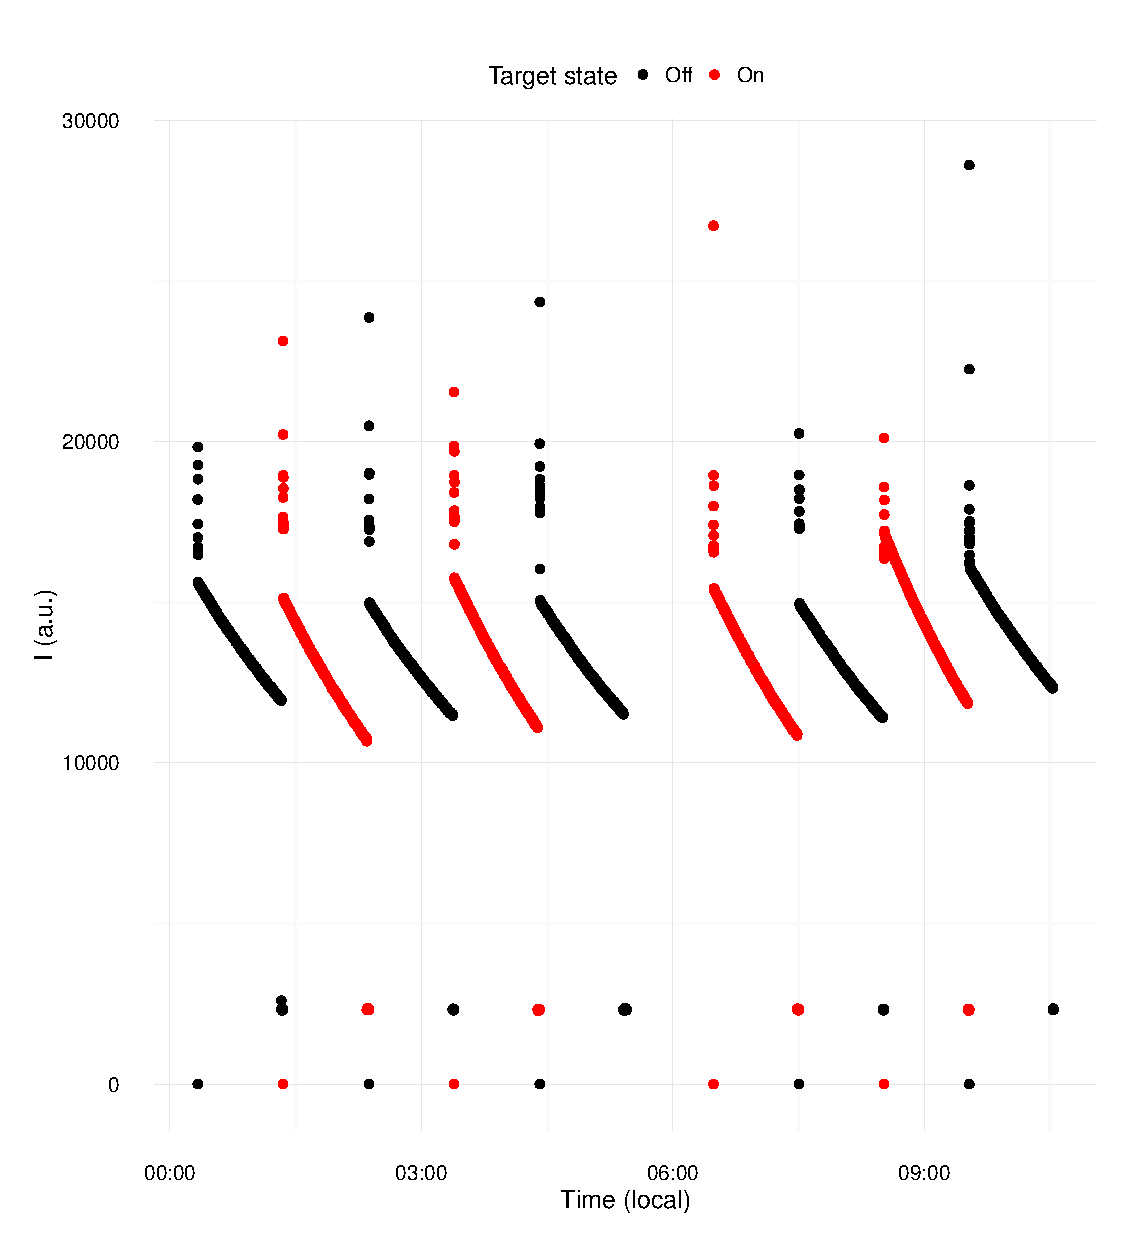
\includegraphics[scale=\scl]{img/Cycles2012.eps}
\caption{Experiment in 2012. The cycles with the target are drawn in red, those without in black.}
\end{subfigure}
\begin{subfigure}{.5\textwidth}
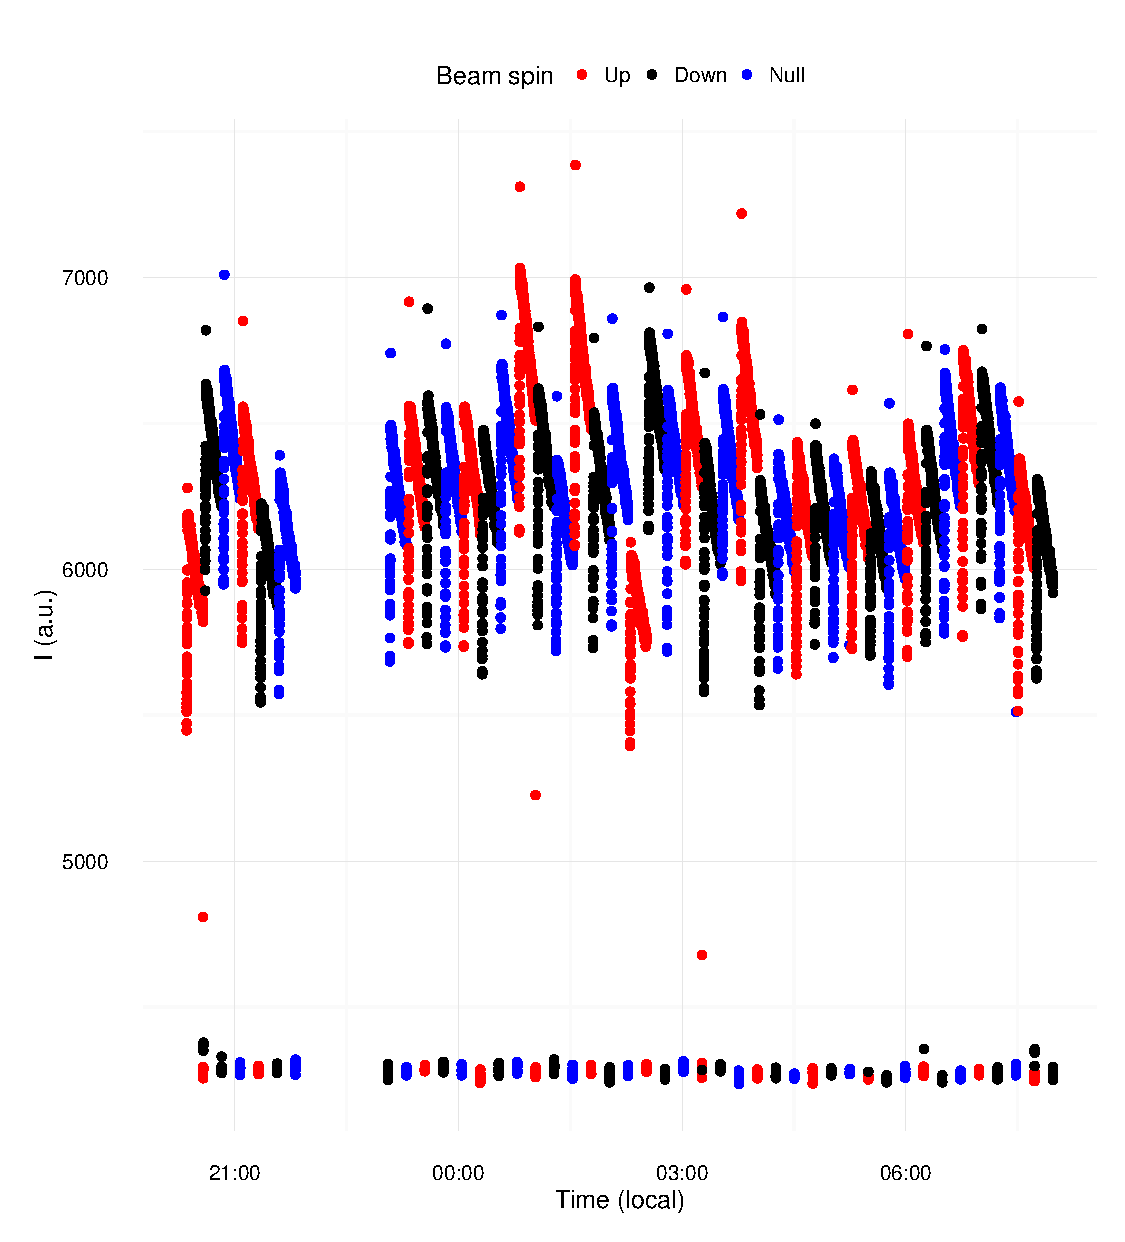
\includegraphics[scale=\scl]{img/Cycles2016.eps}
\caption{Experiment in 2016. The cycles are colored according to the beam spin state.}
\end{subfigure} 
\caption{Average beam current as a function of time.\label{fig:Cycles}}
\end{figure} 


\section{Slope}

In order to correctly estimate a cycle's slope, we subtract the BCT offset $\Delta$ from the data. This is done  because
\begin{align*}
	\tilde{\slp} &= \frac{\td\ln \tilde{I}_t}{\td t} 
				  = \frac{1}{\tilde{I}_t}\frac{\td \tilde{I}_t}{\td t}, 
\shortintertext{where, if the measured current}
	\tilde{I}_t  	&= I_t + \Delta_t = I_0\exp\bkt{\slp\cdot t} + \Delta_t, 
\shortintertext{then}
\tilde{\slp} 	&= \frac{1}{1 + \lambda_t}\bkt{\slp + \frac1{I_t}\frac{\td\Delta_t}{\td t}}, \\
	\lambda_t	&= {I_0}^{-1}\cdot \Delta_t\cdot\exp\bkt{-\slp\cdot t}.
\end{align*}

Even a constant offset must be removed in order to have a constant slope to estimate. The presence of an offset (let alone a time-dependent one) violates the exogeneity assumption, and hence biases the estimate. At this stage, estimation was done assuming offset was constant within a cycle, and its value was estimated as the median of the post-cycle current.

\begin{table}
\centering
\begin{threeparttable}
	\caption{Characteristics of a typical cycle.\label{tbl:CycleChars}}
	\begin{tabular}{llr}
	\hline\hline
	Charactetistic	& Test 					& P-value\\
	\hline
	Linearity 		& Harvey-Collier		& 0\% \\
	-				& Rainbow				& 0\% \\
	Constant slope	& Chow\tnote{a}		 	& 100\% \\
	-				& Moving estimates		& 1\% \\
	Homoskedasticity& Breusch-Pagan 		& 0\% \\
	Autocorrelation & Durbin-Watson			& 0\% \\
	\hline\hline
	\end{tabular}
	\begin{tablenotes}
		\item[a]{The Chow test was performed at every point in the fitting range. The average of F-statistics is used as the test statistic.}
	\end{tablenotes}
\end{threeparttable}
\end{table}

After subtracting the offset, the linear model $\ln I_t = \ln I_0 + \slp t +\epsilon_t$ is fitted via the ordinary least squares method. The reduced chi-squares computed from model residuals deviate from one starting from the fourth decimal place; however, one should note that the data are likely to have structural slope changes, and do not pass linearity tests as well (see TABLE~\ref{tbl:CycleChars}). Because the model residuals exhibit serial correlation (FIG.~\ref{fig:Run969}), the slope estimates' standard errors are estimated with robust estimators. This is done for both data sets.


In FIG.~\ref{fig:SlpOnI0} we plotted the dependence of the slope estimate on the initial beam current, which was estimated by exponentiating the intercept of the fitted model. (If the initial current is also estimated as the median value of current within the second cycle minute, the two estimators are essentially perfectly correlated.) The figure for the 2016 estimates suggests there might be a dependence of the estimated slope on the initial beam current, although the p-values of the slopes of the fitted lines (obtained by robust least squares) are not statistically significant, with only the slope for the null spin state and the target turned off being significant at the 10\% confidence level (the p-value being 6\%). However, one might notice that the effect of the initial current is stronger for the target-off slopes (the difference is especially noticeable in the unpolarized case), affirming the hypothesis that the beam current played a significant role in the experimental performance.

\begin{figure}
\centering
%\begin{subfigure}{.5\textwidth}
%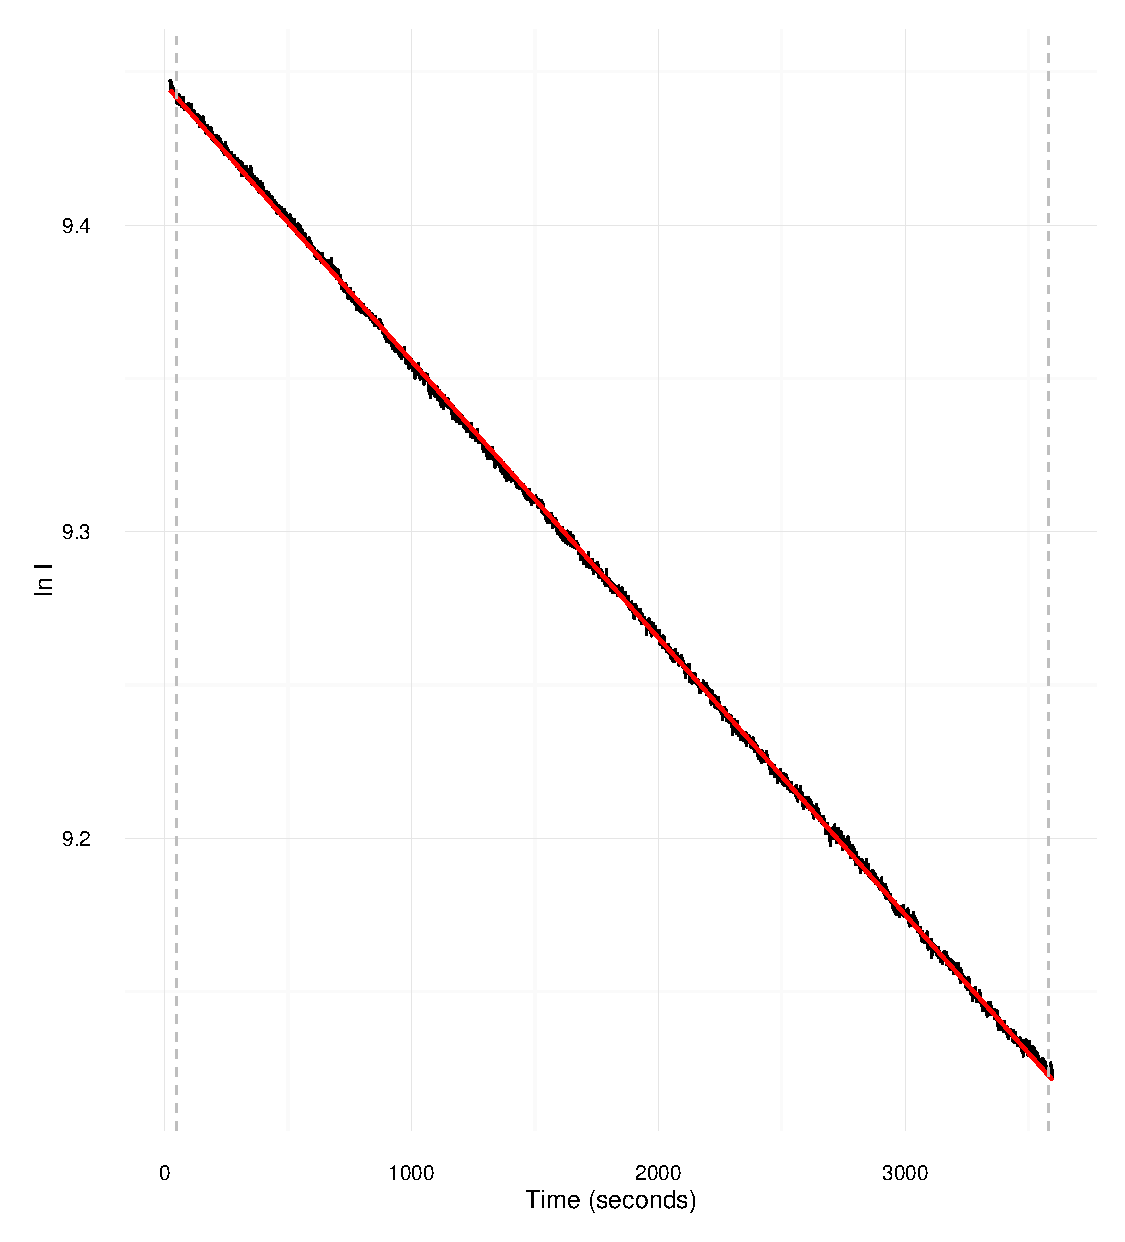
\includegraphics[scale=\scl]{img/Run969_Data_AND_Fit.eps}
%\caption{Logarithm of measurement data as a function of time. The fitted line is colored red, the gray dashed lines mark the fit region.}
%\end{subfigure}
\begin{subfigure}{.5\textwidth}
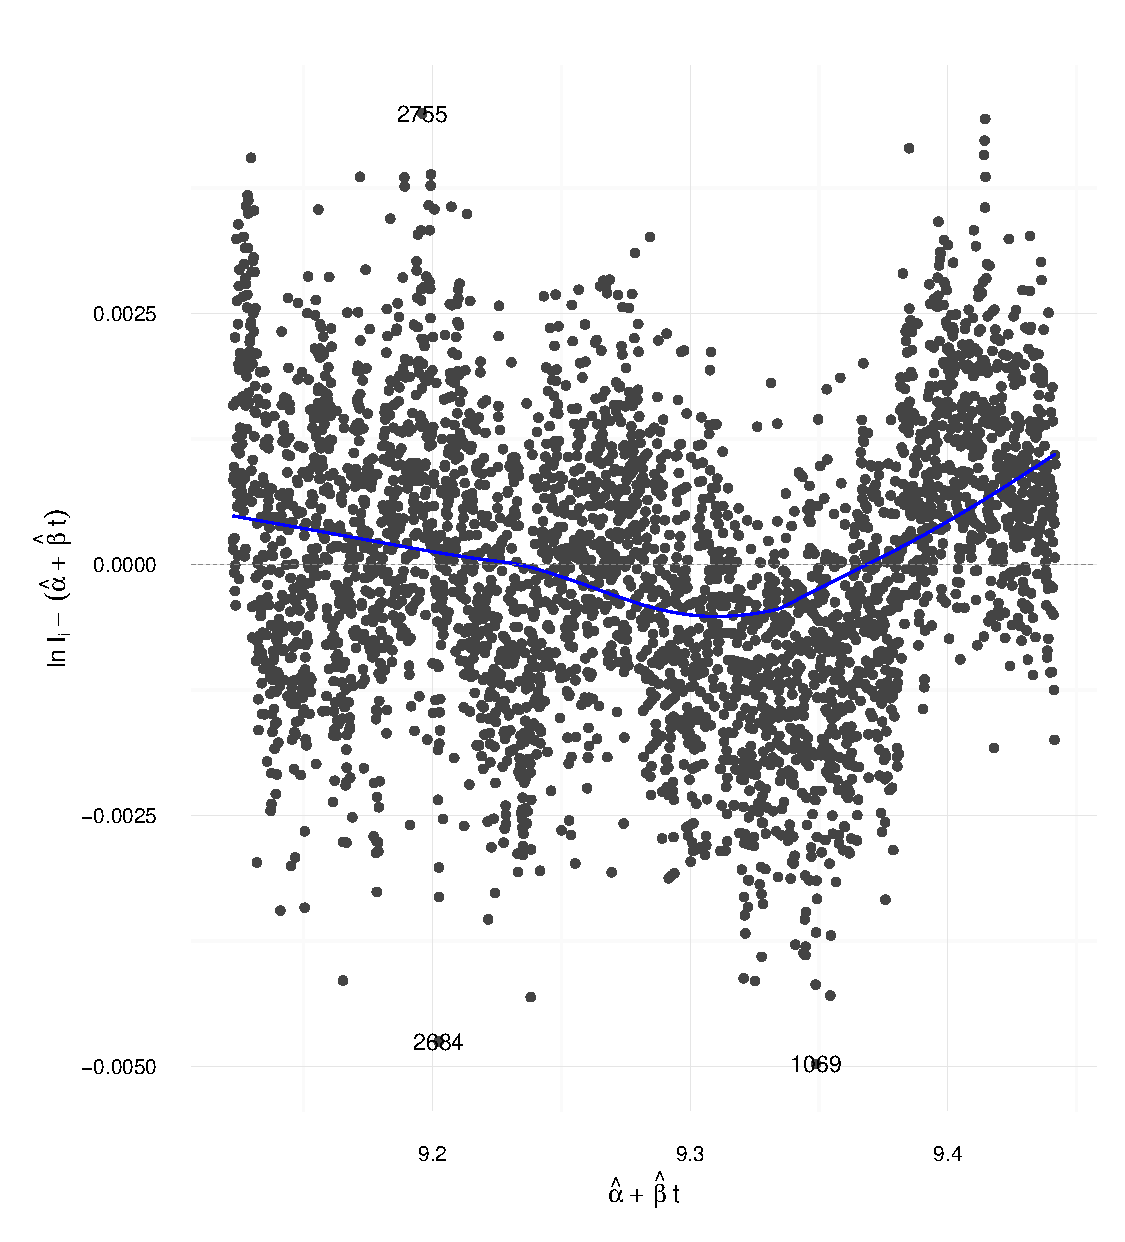
\includegraphics[scale=\scl]{img/Run969_Res_VS_Fit.eps}
\caption{Residuals vs fitted values.}
\end{subfigure}
\begin{subfigure}{.5\textwidth}
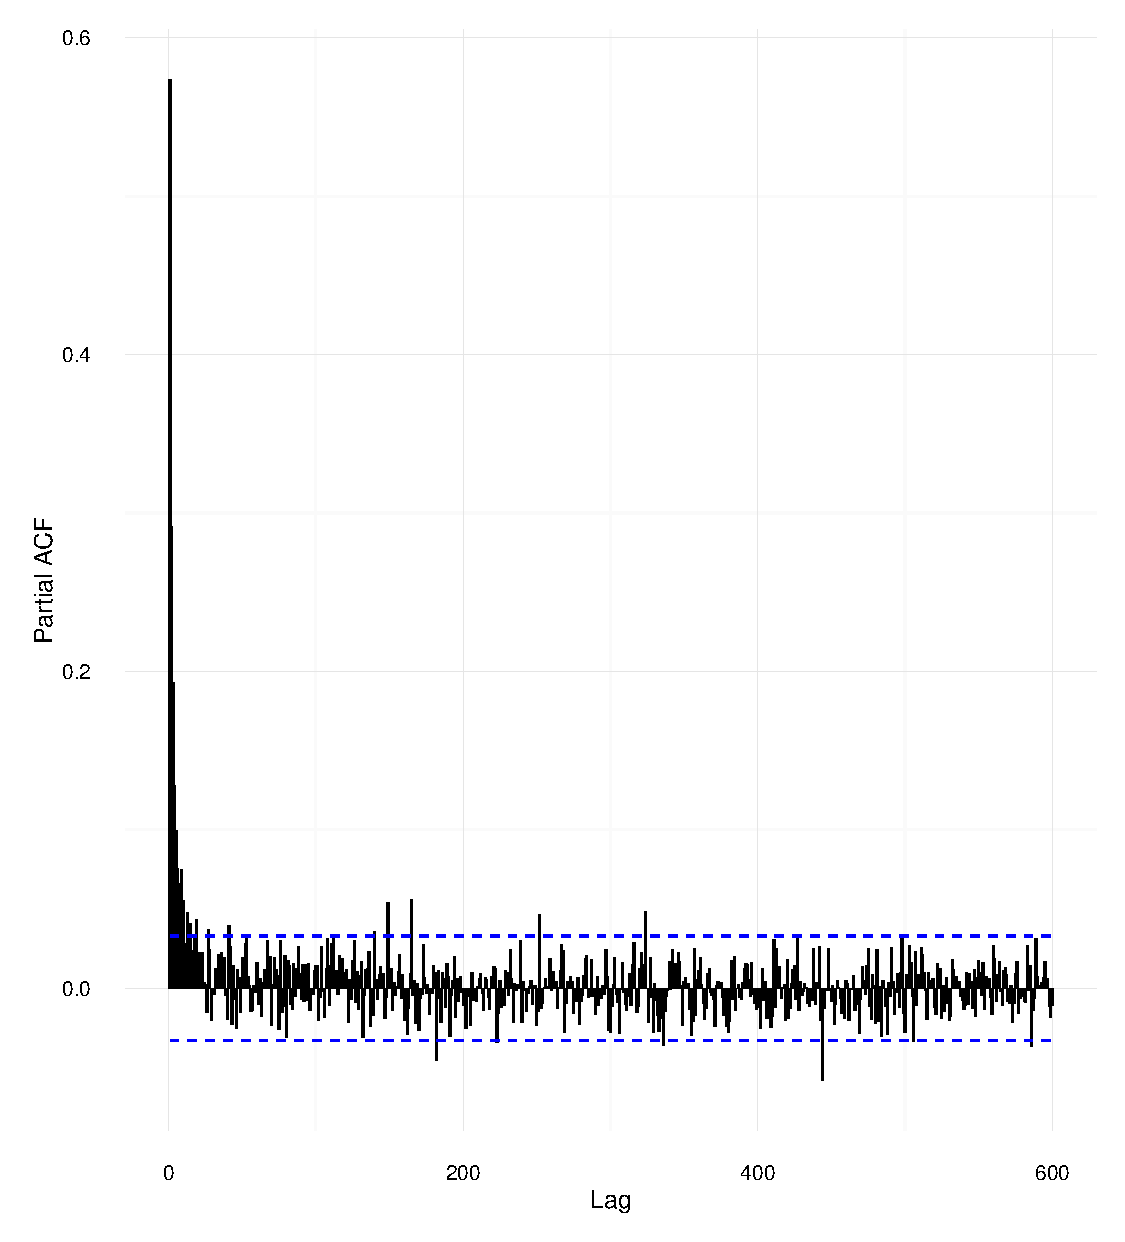
\includegraphics[scale=\scl]{img/Run969_residual_PACF.eps}
\caption{The partial Auto-Correlation Function of the residuals.}
\end{subfigure}
\caption{Some diagnostic plots for a typical cycle.\label{fig:Run969}}
\end{figure}

\section{Cross section}
In estimating the cross section, we used only the estimates from adjacent cycles. This was done to minimize the effect of drifts of environmental variables such as target thickness, which is estimated to increase by $0.5~ \sfrac{\%}{\mathrm{hour}}$. (The thickness by which the slope differences are divided, assumed constant, was provided by a Schottky measurement.) Those estimates whose computation involved at least one slope which does not pass Tukey's range test are labeled unsound.

\begin{figure}
\begin{subfigure}{.5\textwidth}
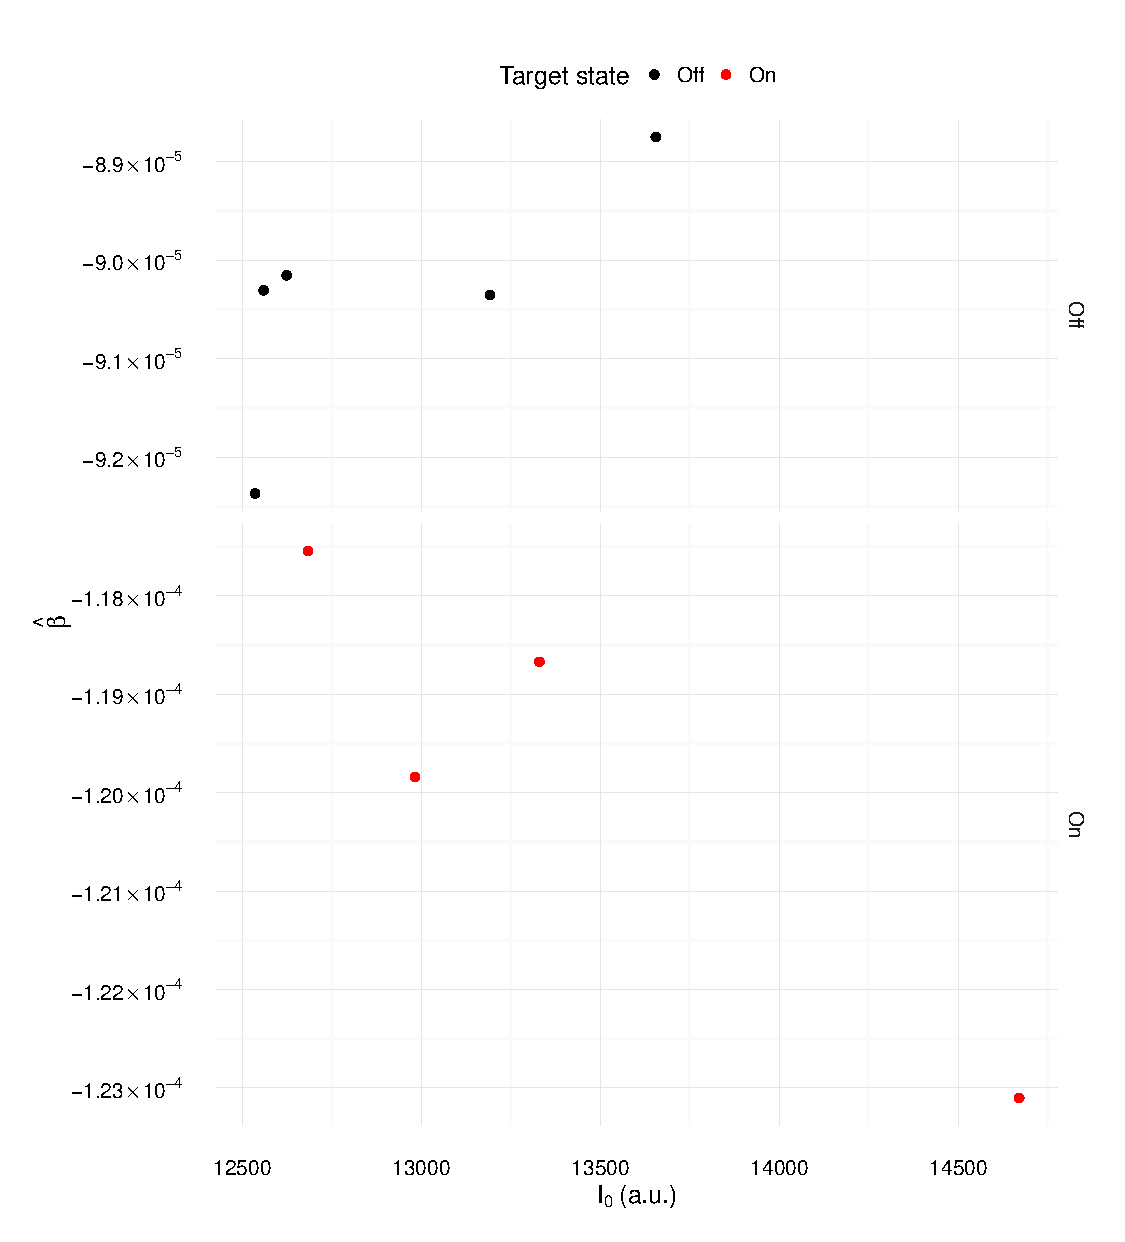
\includegraphics[scale=\scl]{img/Slope_VS_IniCurrent.eps}
\caption{2012.}
\end{subfigure}
\begin{subfigure}{.5\textwidth}
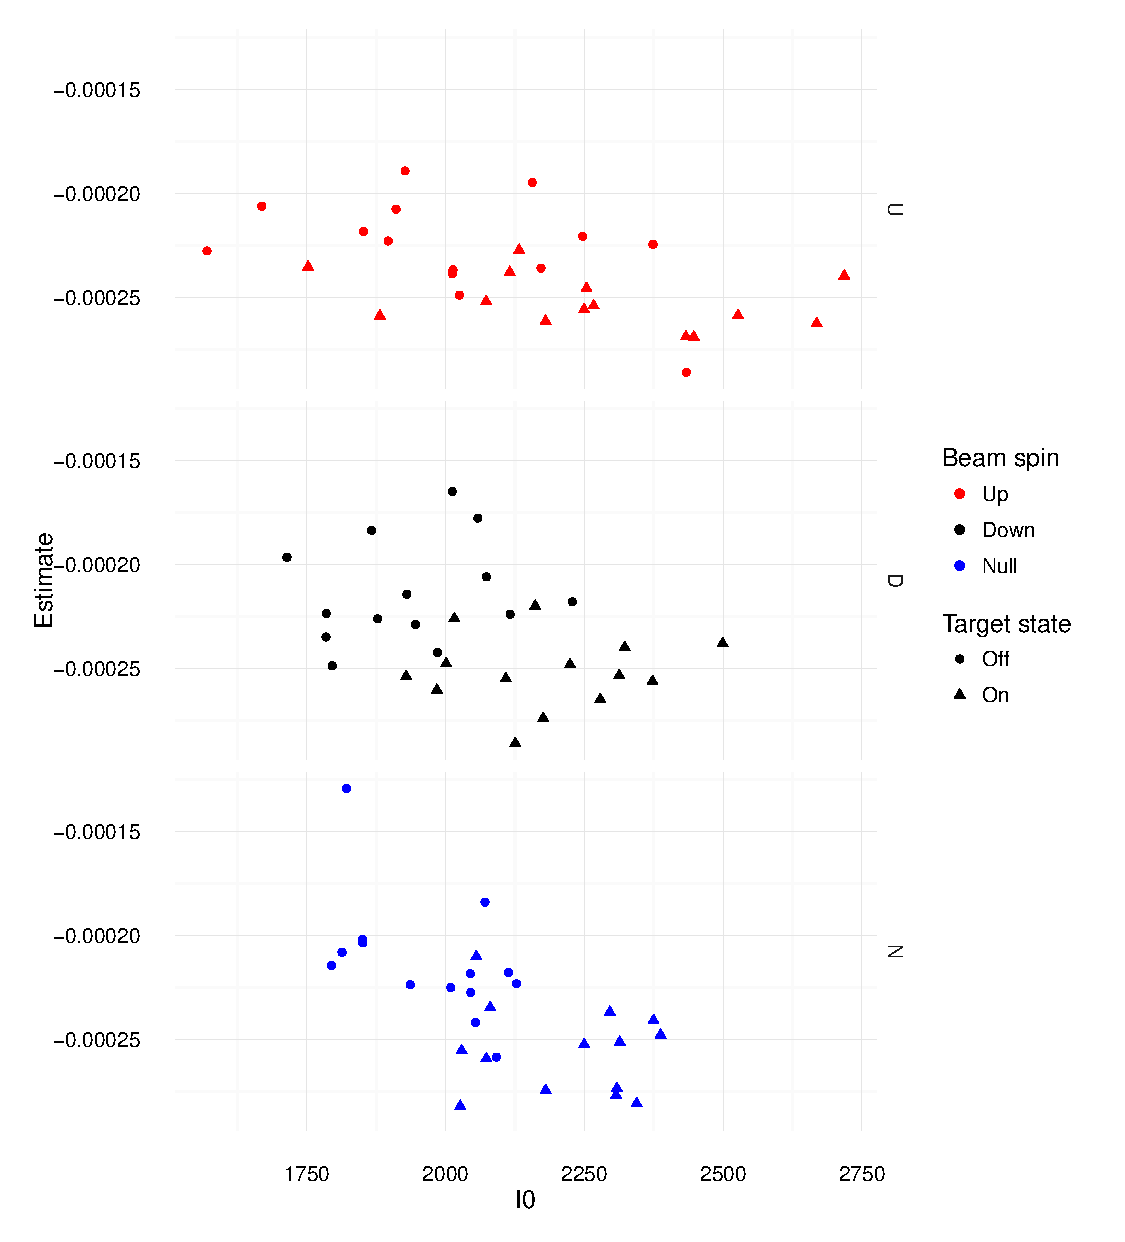
\includegraphics[scale=\scl]{img/Slope_VS_IniCurrent_2016.eps}
\caption{2016.\label{fig:SlpOnI02016}}
\end{subfigure}
\caption{Slope estimates plotted against initial beam current estimated as the exponentiated intercept of the fitted model.\label{fig:SlpOnI0}}
\end{figure}

The cross section estimate's standard error (SE) is estimated by adding the squared standard errors of the paired slopes, not taking account of the covariance term:
\begin{equation}
	\SE*{\CS*[0]} = \sqrt{\SE*{\slp*[off]}^2 + \SE*{\slp*[on]}^2}.
\end{equation}

This is done so because depending on whether an on-slope is paired with the preceding or succeeding off-slope, the covariance term changes sign. Since there does not seem to be a reasonable criterion favoring either of the two mappings, the covariance term was omitted.

\section{Asymmetry}

The asymmetry was estimated as in equation~\eqref{eq:AyyEst}. In that expression, we used the target thickness as estimated using the Schottky measurements method~\cite{Stein} ($1.1\cdot 10^{14}$ cm$^{-2}$), and our own best estimate for the unpolarized cross section (411 mb, see TABLE~\ref{tbl:CS-all}).\\

\section{Results}
\begin{table}
\centering
\begin{threeparttable}
\caption{Cross section summary statistics. \label{tbl:CS-all}}
\begin{tabular}{c|llrcr}
\hline\hline
Year						& Soundness		& Closeness		& \#		& Mean\tnote{a} (a.u.)	& SE (a.u.) \\
\hline
\multirow{4}{*}{2012}		& Sound			& Close			& 4			& 507(507)				& 7  \\
							& Sound			& Far			& 8			& 553(563)				& 14 \\
							& Unsound		& Close			& 3			& 562(580)				& 36 \\
							& Unsound		& Far			& 5			& 515(512)				& 20 \\
							& All			& 				& 20		& 536(544)				& 10 \\
\hline					
\multirow{4}{*}{2016}		& Sound			& Close			& 40		& 409(411)				& 48 \\
							& Sound			& Far			& 92		& 396(385)				& 34 \\
							& Unsound		& Close			& 4			& 1400(1418)			& 170\\
							& Unsound		& Far			& 8			& 1453(1457)			& 69 \\
							& All			& 				& 144		& 486(473)				& 35 \\
\hline\hline
\end{tabular}
\begin{tablenotes}
\item[a] The value in parentheses is the weighted mean with measurements' variance estimates used as weights.
\end{tablenotes}
\end{threeparttable}
\end{table}

The summary statistics of cross section estimates, grouped by soundness and closeness of the slope estimates they are based on, are presented in TABLE~\ref{tbl:CS-all} and FIG.~\ref{fig:CS-all}; the slopes themselves are shown in FIG.~\ref{fig:SlopesVsTime} and summarized in TABLE~\ref{tbl:Slp-big}. Group density estimates with the rectangular kernel are shown in FIG.~\ref{fig:CS-dens}.

\newcommand{\vp}[2]{#1\cdot10^{#2}}
\begin{table}[h]
\centering
\caption{Slope summary statistics. \label{tbl:Slp-big}}
\begin{tabular}{c|lllllrr}
	\hline\hline
	        Year          & Target               & Spin & \# & Mean (a.u.)      & SE (a.u.)    \\ \hline
	\multirow{2}{*}{2012} & Off                  & Null & 5  & $\vp{-9.04}{-5}$ & $\vp{6}{-7}$ \\
	                      & On                   & Null & 4  & $\vp{-1.20}{-4}$ & $\vp{1}{-6}$ \\ \hline
	\multirow{6}{*}{2016} & \multirow{3}{*}{Off} & Up   & 12 & $\vp{-2.26}{-4}$ & $\vp{7}{-6}$ \\
	                      &                      & Down & 12 & $\vp{-2.16}{-4}$ & $\vp{8}{-6}$ \\
	                      &                      & Null & 12 & $\vp{-2.12}{-4}$ & $\vp{9}{-6}$ \\
	                      & \multirow{3}{*}{On}  & Up   & 12 & $\vp{-2.51}{-4}$ & $\vp{4}{-6}$ \\
	                      &                      & Down & 12 & $\vp{-2.53}{-4}$ & $\vp{5}{-6}$ \\
	                      &                      & Null & 12 & $\vp{-2.54}{-4}$ & $\vp{6}{-6}$ 
\end{tabular}
\end{table}

Our best estimate for the $pp$ cross section is $\CS[0]^{pp} = 507 \pm 7$ a.u., that for the $pd$ reaction is $\CS[0]^{pd} = 411 \pm 48$. The asymmetry $\Ayy = \vp{(5 \pm 3)}{-2}$. %FIG.~\ref{fig:AyyDensity} shows its Gaussian kernel density estimate.

%\begin{figure}
%\centering
%	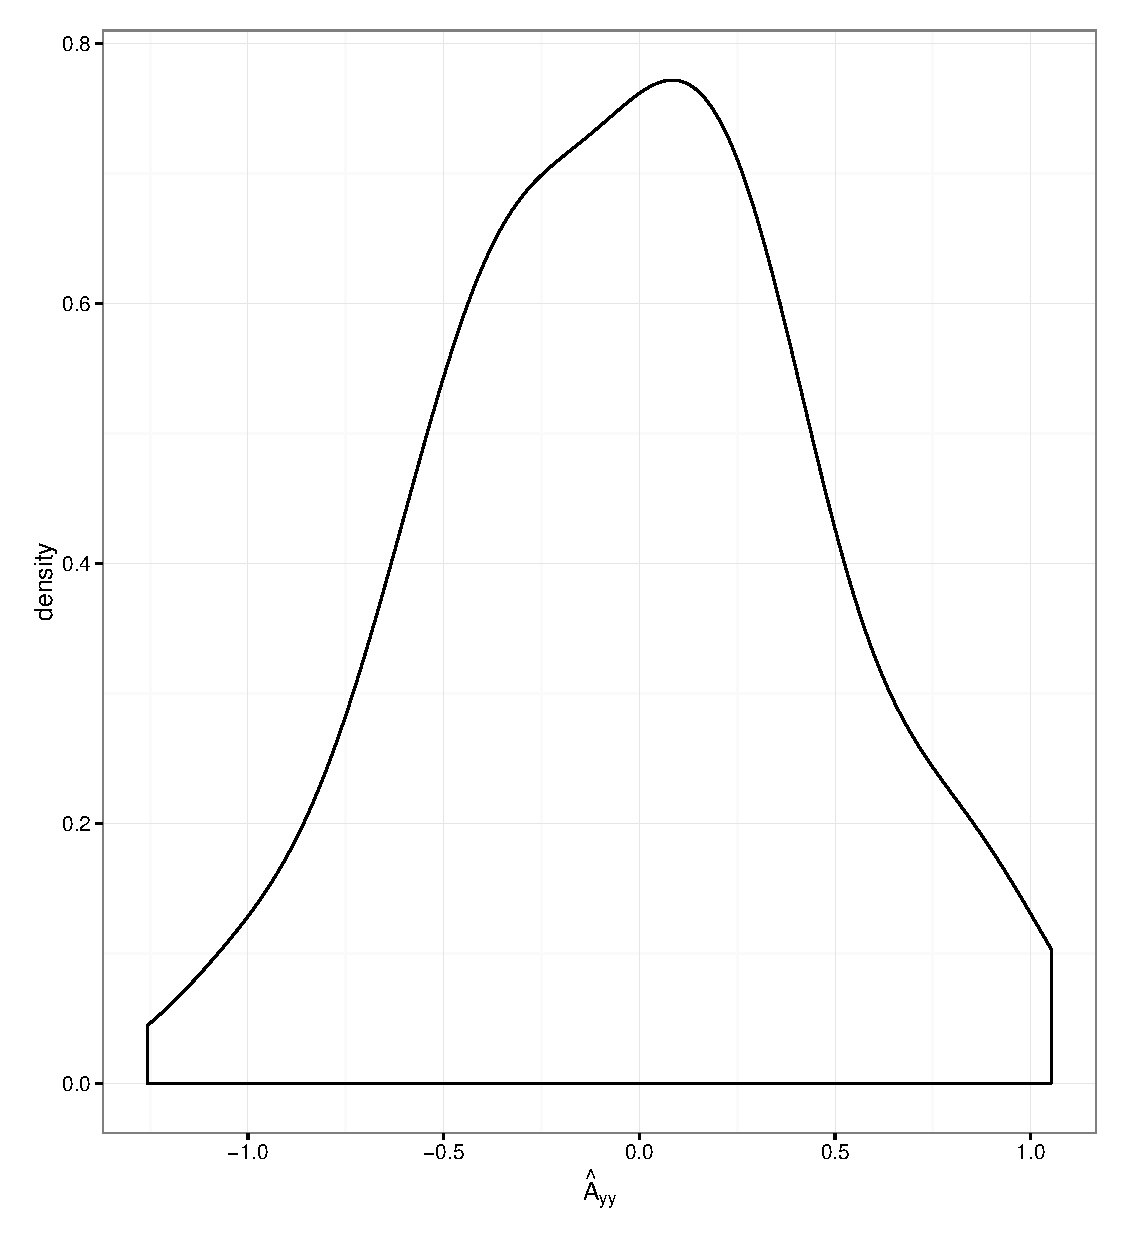
\includegraphics[scale=\scl]{img/Ayy_dens.eps}
%\caption{Gaussian kernel density estimate of the double-polarized cross section asymmetry in proton-deuteron scattering.\label{fig:AyyDensity}}
%\end{figure}

\begin{figure}[t]
\centering
	\begin{subfigure}{.5\textwidth}
		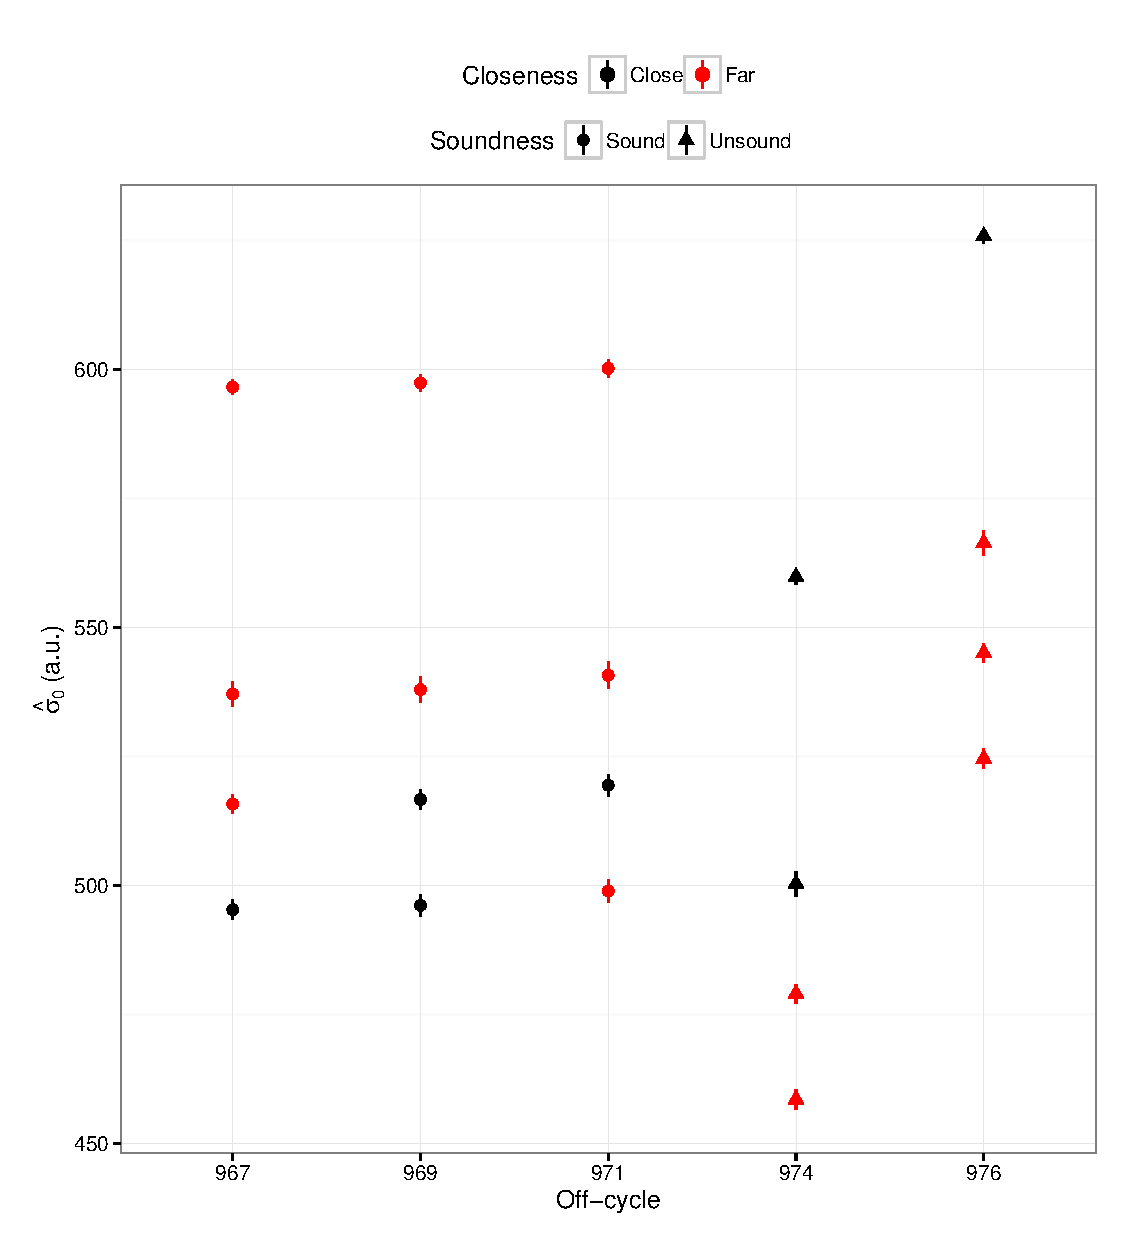
\includegraphics[scale=\scl]{img/Cross-Section2012_all.eps}
		\caption{2012.}
	\end{subfigure}
		\begin{subfigure}{.5\textwidth}
			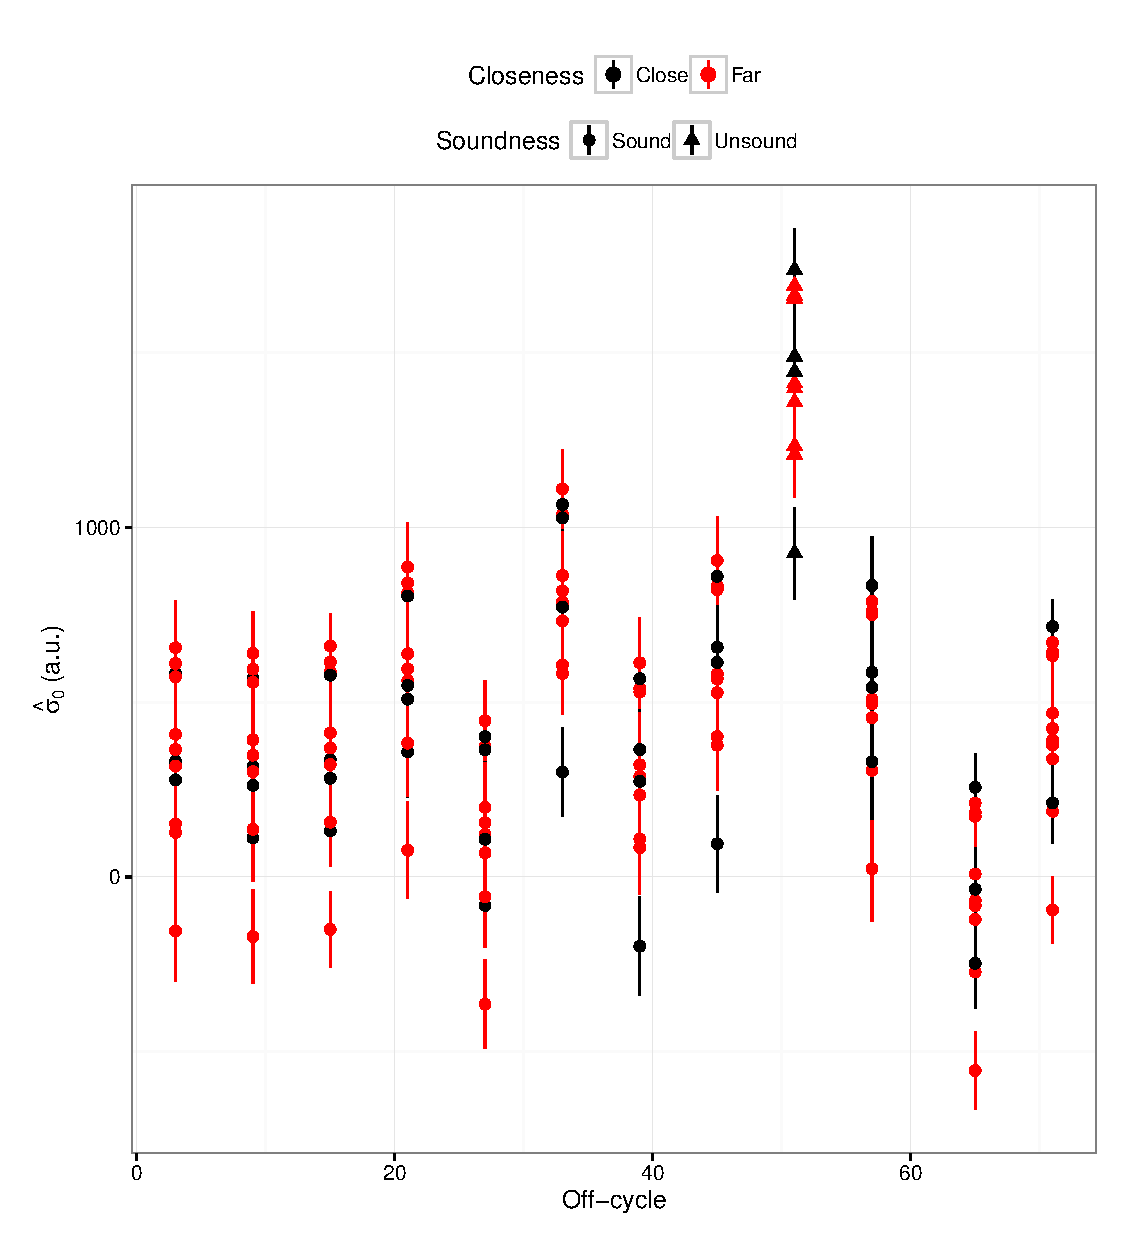
\includegraphics[scale=\scl]{img/CS0mb2016_all.eps}
			\caption{2016.}
		\end{subfigure}
\caption{Cross section estimates plotted against their off-cycle number\label{fig:CS-all}.}
\end{figure}
\begin{figure}
	\centering
\begin{subfigure}{.5\textwidth}
	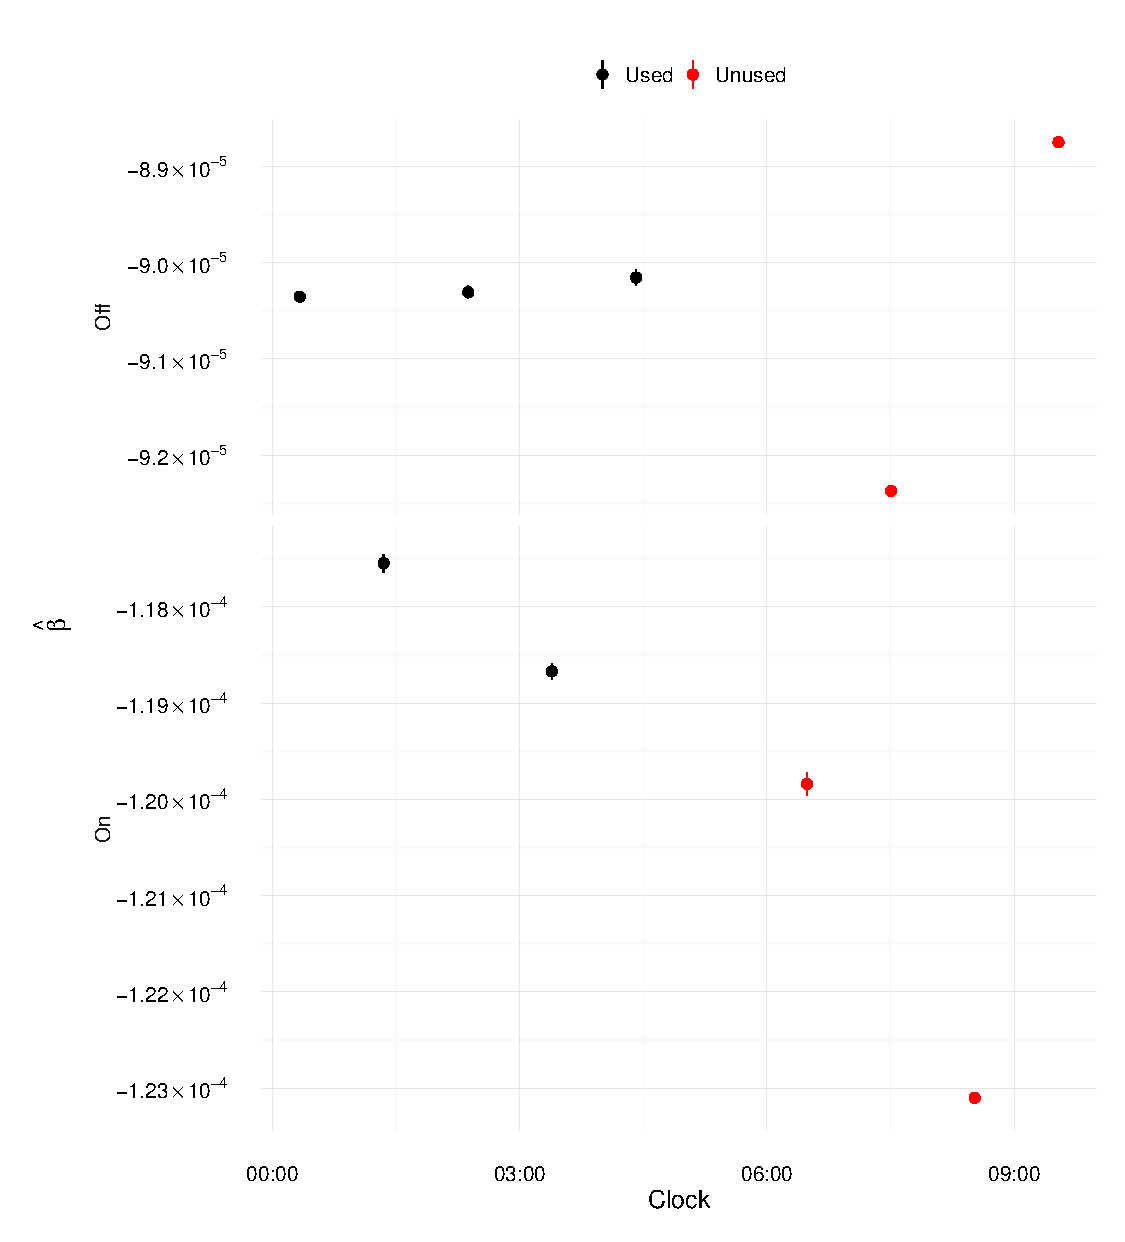
\includegraphics[scale=\scl]{img/Slopes-2012_big.eps}
	\caption{2012.}
\end{subfigure}
\begin{subfigure}{.5\textwidth}
	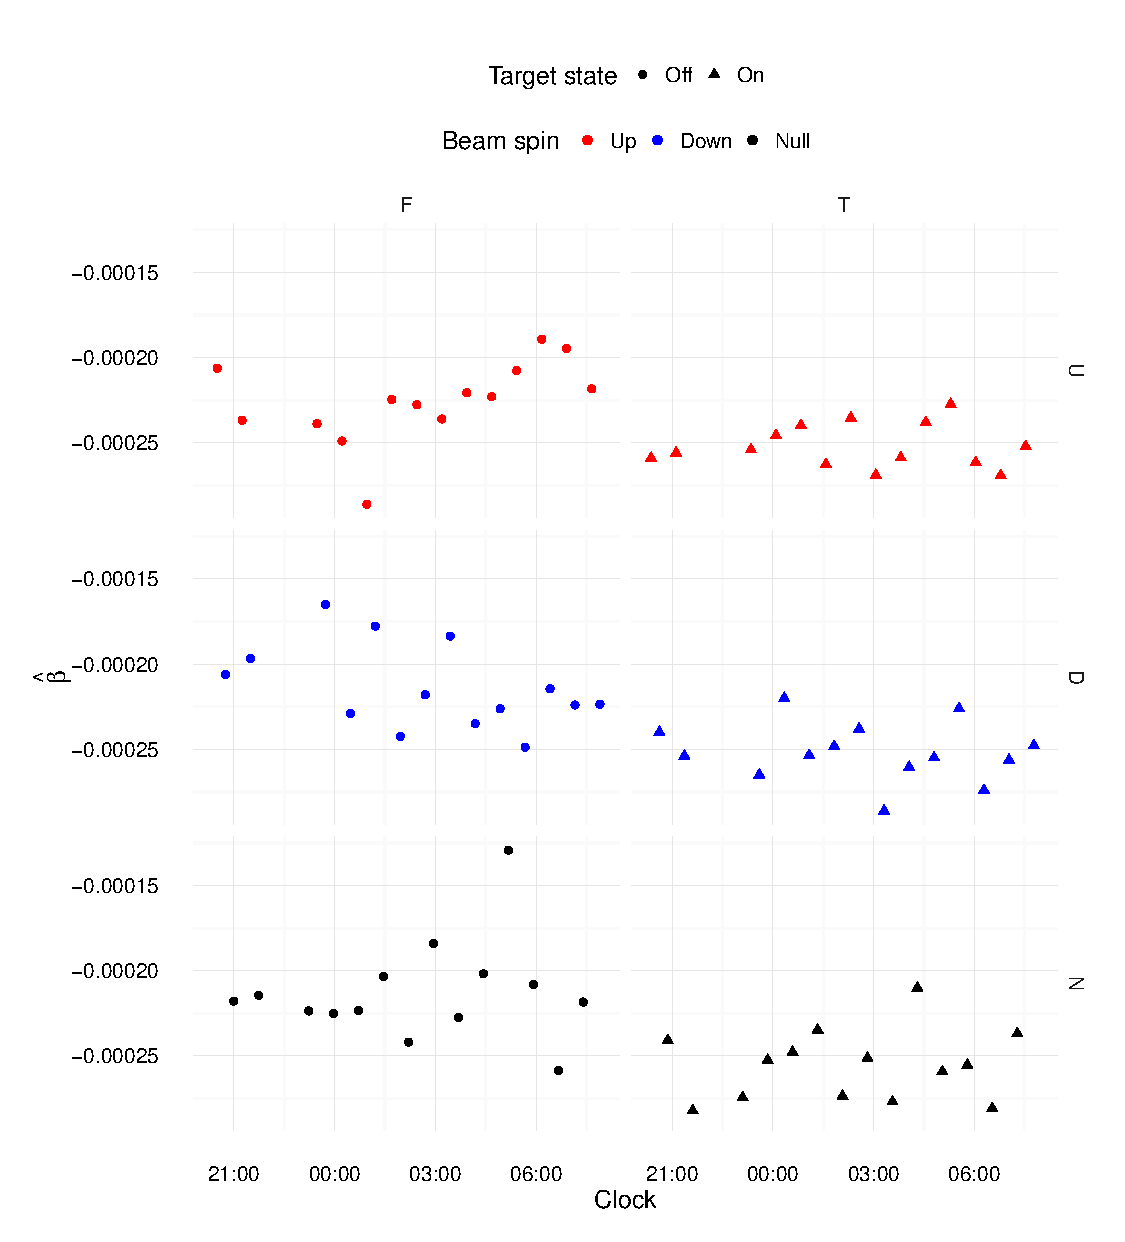
\includegraphics[scale=\scl]{img/Slopes2016_VS_Clock.eps}
	\caption{2016.}
\end{subfigure}
\caption{Slope estimates as a function of time.\label{fig:SlopesVsTime}}
\end{figure}
\begin{figure}
\centering
	\begin{subfigure}[b]{.5\textwidth}
		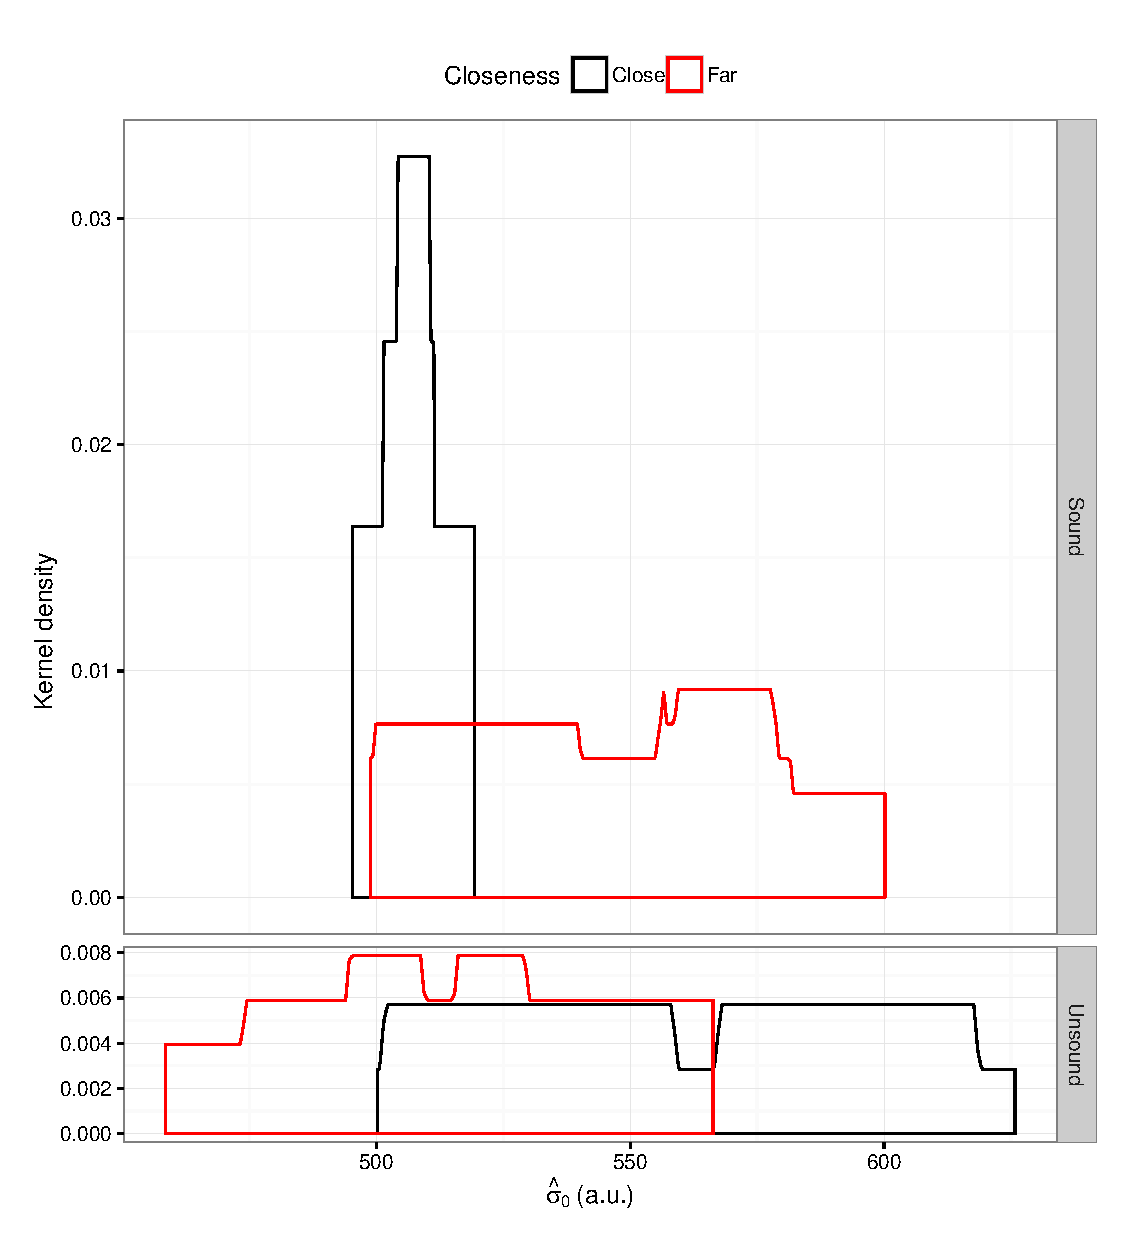
\includegraphics[scale=\scl]{img/Cross-Section2012_dens.eps}
		\caption{2012.}
	\end{subfigure}
	\begin{subfigure}[b]{.5\textwidth}
		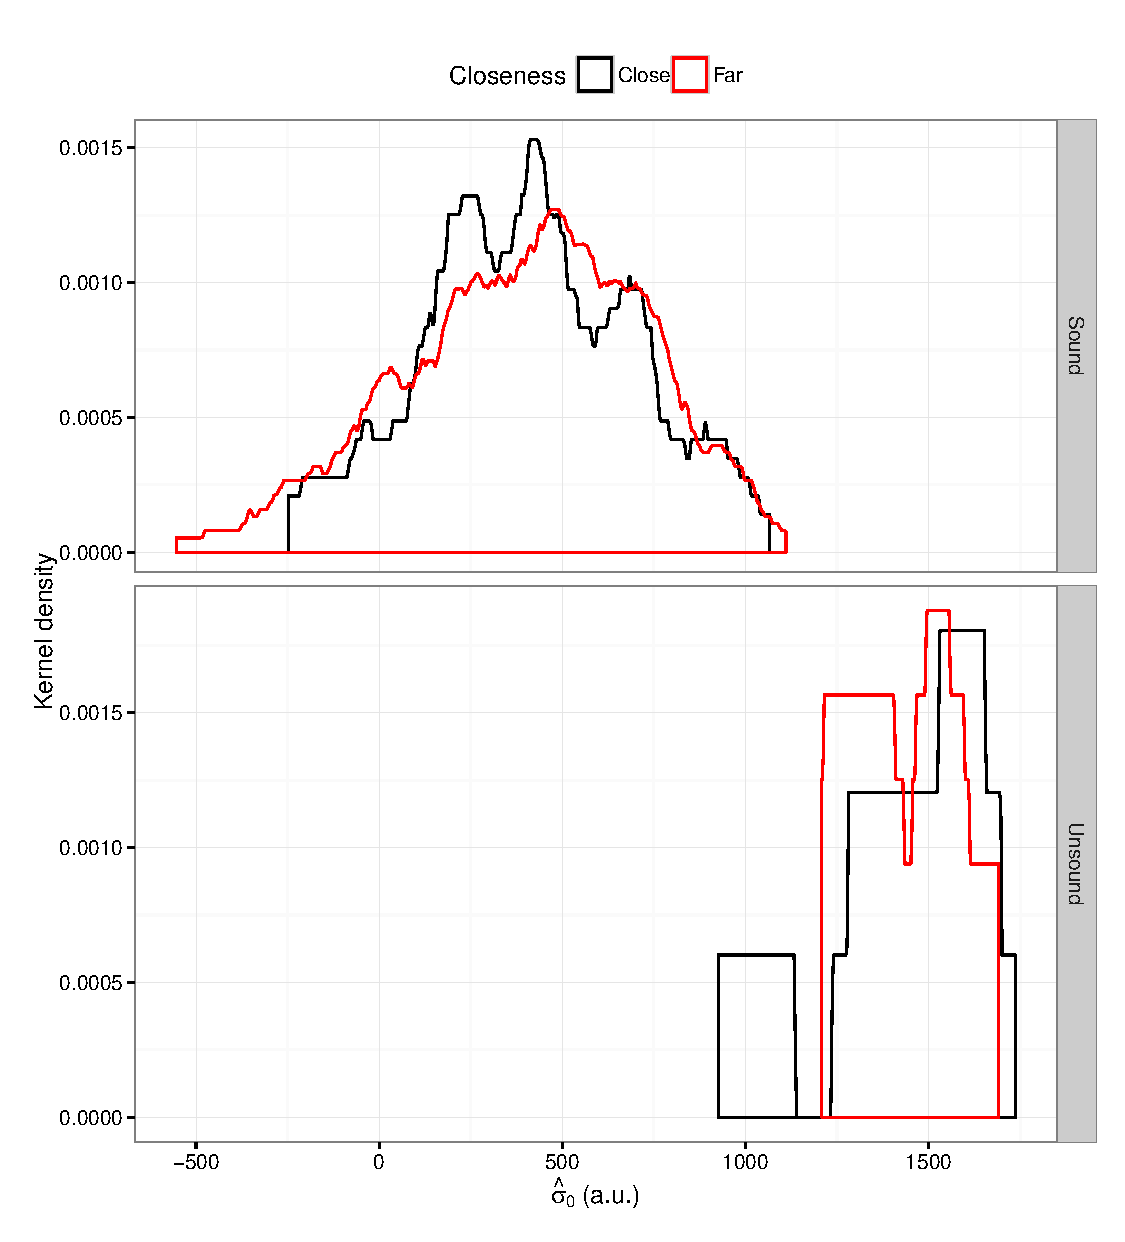
\includegraphics[scale=\scl]{img/CS0mb2016_dens.eps}
		\caption{2016.}
	\end{subfigure}
	\caption{Cross section density estimates for each category of results.\label{fig:CS-dens}}
\end{figure}



\begin{thebibliography}{9}
\bibitem{Conzett}
Homer E. Conzett. ``On Null Tests of Time-Reversal Invariance,'' 6. Paris, France, 1990. %\url{https://publications.lbl.gov/islandora/object/ir%3A93728/datastream/PDF/download/citation.pdf}

\bibitem{Proposal}
P.D. Eversheim, et al. ``Test of Time-Reversal Invariance in Proton-Deuteron Scattering.''
%\url{https://apps.fz-juelich.de/pax/paxwiki/images/8/8c/215-TRI_Prop_sum.pdf}

\bibitem{GaussMarkov}
D.S.G. Pollock. ``Topics in Econometrics.'' %\url{http://www.le.ac.uk/users/dsgp1/COURSES/TOPICS/gausmkov.pdf}

\bibitem{Stein}
H. J. Stein, M. Hartmann, I. Keshelashvili, et al. ``Determination of target thickness and luminosity from beam energy losses.''

\end{thebibliography}

\end{document}
